\documentclass{article}

\usepackage{titlesec}
\usepackage[T1]{fontenc}
\usepackage[utf8]{inputenc}
\usepackage[a4paper,left=3cm,right=2cm,top=2.5cm,bottom=2.5cm]{geometry}
\usepackage{hyperref}
\usepackage{array}
\newcommand{\wiki}[1]{https://pl.wikipedia.org/wiki/Teksel}

\newcommand{\DICOM}[0]{\mbox{DICOM}\xspace}

\def\zerospace{\hspace{0px}}
\def\scopedots{\zerospace::\zerospace}

\def\sokarprefix{Sokar\scopedots}
\newcommand{\sokarclass}[1]{\textit{\sokarprefix#1}}
\newcommand{\sokarfunction}[2]{\textit{\sokarprefix#1\scopedots#2()}}

\def\gdcmprefix{gdcm\scopedots}
\def\gdcmdocurl{http://gdcm.sourceforge.net/html}
\newcommand{\gdcmclass}[1]{\textit{\href{\gdcmdocurl/classgdcm_1_1#1.html}{\gdcmprefix#1}}}
\newcommand{\gdcmfunction}[2]{\textit{\href{\gdcmdocurl/classgdcm_1_1#1.html\##2}{\gdcmprefix#1\scopedots#2()}}}

\def\qtprefix{Qt\scopedots}
\def\qtdocurl{https://doc.qt.io/qt-5}
\newcommand{\qtclass}[1]{\textit{\lowercase{\href{\qtdocurl/#1.html}}{\qtprefix#1}}}
\newcommand{\qtfunction}[2]{\textit{\lowercase{\href{\qtdocurl/#1.html\##2}}{\qtprefix#1\scopedots#2()}}}

\def\stdprefix{std\scopedots}
\newcommand{\stdclass}[2]{\href{https://en.cppreference.com/w/cpp/#2}{\stdprefix#1}}

\newcommand{\dicomvr}[1]{VR:#1}

\def\dicomtagprefix{{\small$^\text{Dicom}_\text{Tag}$}\xspace}
\def\dicomtagurl#1{\url{https://duckduckgo.com/?q=!ducky+#1+site\3Adicom.innolitics.com}}
\newcommand{\dicomtag}[3]{\href{https://duckduckgo.com/?q=!ducky+DICOM+Tag+#1+(#2,#3)+site\%3Adicom.innolitics.com}{\dicomtagprefix#1 (0x#2, 0x#3)}}

\newenvironment{conditions}
{\par\vspace{\abovedisplayskip}\noindent\begin{tabular}{>{$}l<{$} @{${}={}$} l}}
        {\end{tabular}\par\vspace{\belowdisplayskip}}

\def\quotett#1{\enquote{\texttt{#1}}}
\def\cppcode#1{{\color{blue}\texttt{#1}}}
\def\keyword#1{{\textbf{#1}}}
\def\dataword#1{{\color{gray}\enquote{\texttt{#1}}}}

% \renewcommand\paragraph{%
%     \@startsection{paragraph}{4}{0mm}%
%        {-\baselineskip}%
%        {.5\baselineskip}%
%        {\normalfont\normalsize\bfseries}}


\newcommand{\fromEng}[1]{(ang. \textit{#1})}


\newenvironment{infobox}[1][]
{\begin{mdframed}[
            frametitle={#1},
            skipabove=\baselineskip plus 2pt minus 1pt,
            skipbelow=\baselineskip plus 2pt minus 1pt,
            frametitleaboveskip= 7pt,
            frametitlebelowskip= 7pt,
            linewidth=1pt,
            linecolor=black,
            frametitlerule=false,
            frametitlebackgroundcolor=blue!10,
            backgroundcolor=blue!10,
            roundcorner=7pt,
            nobreak=true
        ]}
        {\end{mdframed}}

\newenvironment{zeroindent}
{\par\setlength{\parindent}{0pt}}
{\par}


\def\qtclassExplanations{
    \begin{infobox}
        \begin{zeroindent}
            W dokumencie są wielokrotnie zawarte odniesienia do klas z biblioteki Qt.
            Dlatego, aby zwiększyć czytelność pracy, została zastosowana konwencja poprzedzania klas z biblioteki Qt przedrostkiem \textit{\qtprefix}, który jest za razem przestrzenią nazw.
            Przykład poniżej:

            \begin{center}
                \qtclass{QObject}
            \end{center}

            Wszystkie funkcje wewnątrz klas są oznaczone następująco:

            \begin{center}
                \qtfunction{QObject}{connect}
            \end{center}

            Dodatkowo w dokumencie PDF klikając na nazwę klasy użytkownik zostanie przekierowany do oficjalnej dokumentacji Qt znajdującej się pod adresem \url{\qtdocurl}.
        \end{zeroindent}
    \end{infobox}
}

\def\gdcmclassExplanations{
    \begin{infobox}
        \begin{zeroindent}
            W dokumencie są wielokrotnie zawarte odniesienia do klas z biblioteki GDCM.
            Dlatego, aby zwiększyć czytelność pracy, została zastosowana konwencja poprzedzania klas z biblioteki Qt przedrostkiem \textit{\gdcmprefix}, który za razem jest przestrzenią nazw biblioteki.
            Przykład poniżej:

            \begin{center}
                \gdcmclass{ImageReader}
            \end{center}

            Wszystkie funkcje wewnątrz klas są oznaczone następująco:

            \begin{center}
                \gdcmfunction{ImageReader}{GetImage}
            \end{center}

            Dodatkowo w dokumencie PDF można kliknąć na nazwę klasy i użytkownik zostanie przekierowany do oficjalnej dokumentacji GDCM znajdującej się pod adresem \url{\gdcmdocurl}.
        \end{zeroindent}
    \end{infobox}
}

\def\sokarclassExplanations{
    \begin{infobox}
        \begin{zeroindent}
            W dokumencie są wielokrotnie zawarte odniesienia do klas z przeglądarki obrazów.
            Dlatego, aby zwiększyć czytelność pracy, została zastosowana konwencja poprzedzania klas z aplikacji przedrostkiem \textit{\sokarprefix}, który za razem jest przestrzenią nazw programu.
            Przykład poniżej:

            \begin{center}
                \sokarclass{DataConverter}
            \end{center}

            Wszystkie funkcje wewnątrz klas są oznaczone następująco:

            \begin{center}
                \sokarfunction{DataConverter}{toString}
            \end{center}

            Dodatkowo w dokumencie PDF można kliknąć na nazwę klasy i użytkownik zostanie przekierowany do TU WYMYŚLIĆ DO CZEGO
        \end{zeroindent}
    \end{infobox}
}

\def\dicomtagExplanations{
    \begin{infobox}
        \begin{zeroindent}
            W dokumencie są wielokrotnie zawarte odniesienia do znaczników \DICOM.
            Dlatego aby zwiększyć czytelność pracy, została zastosowana konwencja poprzedzania znaczników przedrostkiem \dicomtagprefix i sufiksem składającym się z numeru grupy i elementu grupy zapisanych heksadecymalnie.
            Przykład poniżej:

            \begin{center}
                \dicomtag{PatientID}{0010}{0020}
            \end{center}

            Oznacza to, że jest to znacznik o słowie kluczowym \enquote{PatientID}, numerze grupy $10_{16}$ i numerze elementu $20_{16}$. 

            Wyrażenie \enquote{informacja ta zawarta w znaczniku \dots} będzie oznaczało, że ta informacja znajduje się w elemencie danych o znaczniku.

            Dodatkowo w dokumencie PDF można kliknąć na nazwę klasy i użytkownik zostanie przekierowany do strony \url{https://dicom.innolitics.com/ciods} poprzez wyszukiwarkę DuckDuckGo, na której znajduje się przeglądarka znaczników \DICOM.
        \end{zeroindent}
    \end{infobox}
}

\def\dicomRetired{
    \begin{infobox}
        \begin{zeroindent}
            Wiele elementów danych lub wartości zostały wycofane ze standardu \DICOM w wersji 3.0.
            Oznaczane są jako wycofane \fromEng{retired}.
            Można dalej wspierać ich obsługę w celach wstecznej kompatybilności, ale nie jest to wymagane.
        \end{zeroindent}
    \end{infobox}
}

\inputencoding{utf8}


\def\utfMaleSign{
\includegraphics[height=1em]{utf8char/malesign.pdf}}
\def\utfFemaleSign{
\includegraphics[height=1em]{utf8char/femalesign.pdf}}


\author{Adam Jędrzejowski}
\title{Wieloplatformowa przeglądarka obrazów DICOM w C++}
\date{\today}

\begin{document}

\maketitle

cel pracy

rozdził wprowadzenie

obrazowe techniki diagnostyczne

coto są obrazy diagnostyczne, jakie one mogą być

jakie cechy posinna spełniać przglądrka obrazów

dlaczego tworzymy wieloplatformową w c++

Układ pracy

\part{Wstęp}
\section{Techniki obrazowania medycznego}
\label{MedicalDiagnostics}

W różnych technikach obrazowania, obraz powstaje w jakiś konkretny sposób

Jeżeli diagnozujemy pacjent bądź obiekt, zazwyczaj chcemy zapisać wynik naszej diagnozy/badania.
techniki


\section{Wiadomości ogólne o przeglądarkach obrazów DICOM}

\subsection{Standard DICOM}

Transfert Syntax?
Conformance Statment?

\subsection{Zakres możliwość przeglądarek}

Przeglądarki to jest jeden z rodzajów oprogramowania używanego w obrazowaniu medycznym

Przetwarzanie
Analiza
Mierzenia

Czym rózni się od wybou medycznego

Każda dostępna przeglądarka na rynku, zarówno OpenSourcowym jak i komercyjnym jest inna niepowtarzalna.
Ale można wypunktować pewne cechy wspólne ich Możliwości:

\begin{itemize}
    \item Wyświetlanie obrazu
    \begin{itemize}
        \item powiększenie
        \item obrót
        \item przesuniecie
        \item skalowanie
    \end{itemize}
    \item Analiza obrazu
    \begin{itemize}
        \item Rekonstrukcja 3D z sekwencji obrazów
    \end{itemize}
\end{itemize}


\subsection{Określenia możliwość mojej przeglądarki}

Obsługa DIOCM

Modalności

Typy obrazu


\subsubsection{Wspierane typu obrazów}

W bazie danych tag \dicomtag{Photometric Interpretation}{0028}{0004} określa w jaki sposób należy interpretować wartość piksela w obrazie.
W standardzie zdefiniowano 13 różnych przestrzeni barw \dicomtag{Photometric Interpretation}{0028}{0004} z czego używanych jest tylko 5.

\begin{itemize}
    \item Monochrome1

    Skala szarości, w której 0 oznacza biel a wartość maksymalna(definiowana przez inny parametr) czerń.

    \item Monochrome2

    Skala szarości, w której 0 oznacza czerń a wartość maksymalna(definiowana przez inny parametr) biel.

    \item RGB

    Najbardziej rozpoznawana przestrzeń barw, składająca się z kanałów czerwonego, zielonego i niebieskiego

    \item Palette Color

    Tego nie wspieram na razie, bo nie ograniam jak to działa

    \item YBR Full


    \item Niewspierane
    \begin{itemize}
        \item HSV - \textit{retired}, dosłownie z angielskiego, emerytowany, modalność,
        \item ARGB - \textit{retired}
        \item CMYK - \textit{retired}
        \item Pochodne YBR
        \begin{itemize}
            \item YBR Full 422
            \item YBR Partial 422
            \item YBR Partial 420
            \item YBR ICT
            \item YBR RCT 
        \end{itemize}
    \end{itemize}

\end{itemize}

\subsubsection{Jak będzie pokazywany obraz}

\subsubsection{Sposób wyświetlania}

Kino

\subsubsection{Obsługa błędów}

Standard DICOM był zaprojektowany w ten sposób, aby mógł być poszerzany o nowe parametry w przyszłości, oraz tak aby ten nowe parametry nie ingerowały w strukturę już istniejących


\part{Standard DICOM}

\part{Biblioteki}

\part{Interfejs graficzny}

\part{Implementacja}

\section{Wieloplatformowość}
Przeglądarka jest napisana w taki sposób, że jej implementacja nie uwzględnia systemu operacyjnego na którym pracuje

Zróżnych perspektyw

\subsection{Język programowania}

Przeglądarka została napisana w C++ w standardzie z 2017 roku w skrócie C++17

\subsection{Środowisko programistyczne}

Do programowania głównie używałem CLion, IDE stworzonego przez firmę JetBrians.
Zdecydowaną większość czasu przeglądarka była testowana i debugowana na aktualizowanym systemie ArchLinux.

\subsection{Obiektowy model w oprogramowaniu}

Praca jest zaprojektowany w sposób obiektowy, za wyjątkiem kilku pomniejszych elementów.

\section{Konwertowanie i analiza danych w tagach}

Każdy plik DICOM posiada \quotett{Data Set}, czyli zbiór informacji składający się z \quotett{Data Element}.
\quotett{Data Element} jest strukturą przechowującą wszystkie dane dotyczące obrazu.

\paragraph{Budowa \textquote{Data Element}}

\begin{itemize}
    \item Data Element Tag - to unikalny identyfikator, złożony z dwóch liczb: grupy(uint16) i elementu(uint16) grupy.
    Obiekt używany do przechowywania taga to \gdcmclass{Tag}.
    Informuje o znaczeniu danych.
    Na przykład: jeżeli tag przyjmie wartość \dicomtag{PatientName}{0010}{0010}, oznacza to, że dane w \textquote{Data Element} zawierają nazwę pacjenta.
    \item Value Representation, w skrócie VR – typ danych umożliwiający poprawną interpretację danych.
    Informuje w jaki sposób dane są zapisane.
    Obiekt używany do przechowywania taga to \gdcmclass{VR}.
    Na przykład: Decimal String, w skrócie DS, oznacza liczbę zapisaną za pomocą teksu.
    Czasami to pole może być puste, wtedy należy się odnieść do VR przypisanego do taga, który określa standard.
    \item Value Length, w skrócie VL – rozmiar elementu
    \item Value Field (opcjonalne) – pole z właściwymi danymi
\end{itemize}

\paragraph{Konwerter}

Obiekt klasy \sokarclass{DataConverter} to obiekt zajmujący się konwersją danych z pliku DICOM na dane w formacie odpowiadającej przeglądarce.

Kilka rzeczy które się tyczą wszystkich danych i konwersji:
\begin{itemize}
    \item większość VR jest to zapisane jako tekst, kodowanie i dekodowanie tekstu jest zapewniane przez bibliotekę, a konkretniej przez klasę \gdcmclass{StringFilter}, dlatego nie przejmuje się takimi rzeczami jak zapisem LittleEndian i BigEndian.
    \item większość danych może mieć kilka wartości oddzielonych backslashem \quotett{\textbackslash}, dlatego konwerter dla VR w, których standard przewiduje wiele wartości, zawsze zwraca \qtclass{QVector} z tymi wartościami
    \item wszystkie dane są zapisane parzystą ilością bajtów, w przypadku tekstu dodaje się znak spacji na końcu danych, taka spacja jest pomijana w analizie danych
\end{itemize}

Klasa obsługuje następujące VR:
\begin{itemize}
    \item AS - Age String - wiek lub długość życia

    Długość danych zawsze wynosi 4 bajty.
    Pierwsze trzy bajty to liczba całkowita zapisana za pomocą tekstu.
    Czwarty bajt to znaku określający jednostkę czasu.
    Standard definiuje cztery możliwe jednostki czasu: \quotett{D} jako dzień, \quotett{W} jako tydzień, \quotett{M} jako miesiąc, oraz \quotett{Y} jako jeden rok.
    Konwerter zmienia tą wartość na tekst w postaci czytelnej, np: \quotett{18 weeks} lub \quotett{3 years}, oraz jest wrażliwy na obecny język aplikacji.
    
    Przykład: \quotett{018M} oznacza 18 miesięcy, \quotett{123D} oznacza 123 dni.

    \item AT - Attribute Tag - inny tag

    Długość danych to zawsze 32 bity, są to dwie 16 bitowe liczby.
    Odpowiednio grupa i element grupy.
    Ten VR jest używany kiedy wskazujemy na inny tag.
    Wartość nie jest nigdy pokazywana użytkownikowi, a jedynie używana w interpretacji przez algotyrm tworzenia filmu.
    
    Przykład: tag \dicomtag{FrameIncrementPointer}{0028}{0009} jest używany kiedy w pliku jest zapisana sekwencja kilku obrazów, wskazuje on na inny tag zawierający informacje w jaki sposób ta sekwencja ma być wyświetlona.
    
    \item DA - Date - data lub dzień

    Długość danych zawsze wynosi 8 bajtów.
    Data zapisana w formacie \quotett{YYYYMMDD}, gdzie: \quotett{YYYY} cztery cyfry roku, \quotett{MM} dwie cyfry miesiąca, \quotett{DD} dwie cyfry dnia w kalendarzu Gregoriańskim.
    Konwerter zamienia dane na obiekt klasy \qtclass{QDate}, który ma w sobie wbudowaną konwersję na tekst zależny od ustawień językowych aplikacji.
    
    Przykład: \quotett{19800716} oznacza 16 lipca 1980
    
    UWAGA: Standard \quotett{ACR-NEMA Standard 300}, czyli poprzednik DICOM definiował date w sposób \quotett{YYYY.MM.DD}, według standardu DICOM, taki zapis jest nie poprawny, ale zdarzają się stare obrazy z takimi datami i \sokarclass{DataConverter} obsługuje taki format.

    \item DS - Decimal String - liczba zmienno przecinkowa lub ciąg kilku liczb zmienno przecinkowych zapisanych za pomocą tekstu w notacji wykładniczej

    Długość jednej liczby powinna maksymalne wynosić 16 bajtów.
    Dostępne znaki to \quotett{0}-\quotett{9}, \quotett{+}, \quotett{-}, \quotett{E}, \quotett{e}, \quotett{.}.
    Biblioteka QT posiada wbudowany konwerter liczb zapisanych w formacie wykładniczym, dlatego mój konwerter dzieli tekst i konwertuje za pomocą QT.
    
    Przykład: \quotett{426\textbackslash468 } oznacza dwie liczby 426 i 468. Proszę zwrócić uwagę na spacje na końcu.

    \item IS - Integer String - liczba całkowita 

    Długość jednej liczby powinna maksymalne wynosić 12 bajtów.
    Dostępne znaki to \quotett{0}-\quotett{9}, \quotett{+}, \quotett{-}.
    Biblioteka QT posiada wbudowany konwerter liczb całkowitych, dlatego mój konwerter używa konwertera z QT.
    
    Przykład: \quotett{426 }  oznacza liczbę 426.

    \item PN - Person Name - nazwa osoby

    Jako, że pacjenta, bądź obiekt badany można nazwać w sposób dowolny i odbiegający od polskiego standardu nazewnictwa, standard DICOM nie przewiduje rozdzielenie poszczególnych składowych nazwy na oznaczone fragmenty.
    \quotett{Person Name} dzieli nazwę na podane fragmenty, rozdzielony znakiem \quotett{\^{}} (94 znak kodu ASCII):
    \begin{itemize}
        \item family name complex - nazwisko, np. Smolik
        \item given name complex - imię, np. Adam
        \item middle name - środkowe imię, brak odpowiednika w polskim nazewnictwie
        \item name prefix - prefiks przed imieniem, np: mgr. inż.
        \item name suffix - sufiks po imieniu, brak odpowiednika
    \end{itemize}
    Długość jednego fragmenty powinna maksymalne wynosić 64 znaki.
    W przypadku mniejszej ilości segmentów, mamy założyć, że są puste.
    
    Przykład: \quotett{prof. dr. hab. inż. Waldemar Smolik pracownik ZEJIM} był by zapisany w sposób następujący: \quotett{Smolik\^{}Waldemar\^{}\^{}prof. dr. hab. inż.\^{}pracownik ZEJIM}

    \item SS - Signed Short - 16 bitowa liczba całkowita bez znaku
    
    Jako, że biblioteka GDCM zajmuje się konwersją Little i Big Endian, mogę dane zinterpretować jako typ \quotett{quint16}

    \item US - Unsigned Short - 16 bitowa liczba całkowita ze znakiem

    Jako, że biblioteka GDCM zajmuje się konwersją Little i Big Endian, mogę dane zinterpretować jako typ \quotett{qint16}
    
    \item UT - Unlimited Text - tekst o nieograniczonej długości.

    Zwykły tekst o długości maksymalnie 2\textsuperscript{32}-2 bajtów.
\end{itemize}

\section{DicomScene}

Jest to obiektem jednej ramki obrazu i jest odpowiedzialna za pośrednie wygenerowanie obrazu oraz jego wyświetlenie na ekranie.
Klasa dziedzicząca pośrednio po \qtclass{QGraphicsScene} przez \sokarclass{Scene}.

\subsection{Informacje wyświetlane na scenie}
Informacje na obrazie są wyświetlane za pomocą obiektów \sokarclass{SceneIndicator}.
Obiekty te mają dostęp do bazy danych obrazu DICOM i odpowiednio zmieniają swoją zawartość.

Domyślnie obiekty wyświetlające informacje:
\begin{itemize}

    \item \sokarclass{PatientDataIndicator}

    Obiekt wyświetlający dane pacjenta, pojawia się od zawsze na obrazie w lewym górnym rogu i zawiera następujące linie:
    \begin{itemize}
        \item Nazwa pacjenta oraz płeć

        Nazwa pacjenta znajduje się w \dicomtag{PatientName}{0010}{0010} o \dicomvr{PN}.
        
        Płeć, zapisana jest w \dicomtag{PatientSex}{0010}{0040} i może mieć następujące wartości:
        \begin{itemize}
            \item \quotett{M } - oznacza mężczyznę, wyświetlana jako O
            \item \quotett{F } - oznacza kobietę, wyświetlana jako O
            \item \quotett{O } - oznacza inną płeć i nie jest wyświetlana
        \end{itemize}
        
        W przypadku określenia inne płci niż jest w standardzie bądź braku tagu płeć nie będzie widoczna.

        Przykład: \quotett{Adam Jędrzejowski O}.

        \item Identyfikator pacjenta

        Unikalny identyfikator pacjenta z tagu \dicomtag{PatientID}{0010}{0020} wyświetlane w takiej formie jakiej jest zapisane, bez żadnej obróbki.
        W praktyce najczęściej jest to numer z systemu używanego w danym szpitalu, rzadziej numer pesel.
        
        Przykład: \quotett{HIS/000000}.

        \item Data urodzenia oraz wiek pacjenta w trakcie badania

        Data urodzenia znajdująca się w \dicomtag{PatientBirthDate}{0010}{0030} i jest zamieniana na format \quotett{YYYY-MM-DD}.
        Dodatkowo, jeżeli tag \dicomtag{PatientAge}{0010}{1010} jest obecny wyświetlany jest także wiek pacjenta w czasie badania.
    
        Przykład: \quotett{born 1982-08-09, 28 years}.

        \item Opis wykonany przez instytucję opis lub klasyfikację badania (komponentu)
        
        Tekst brany z \dicomtag{StudyDescription}{0008}{1030} i wyświetlany bez żadnej obróbki.

        UWAGA: Ta wartość jest wpisywana przez technika, operatora lub lekarza wykonującego badanie, więc wartość ta może być nie przewidywalna.

        \item Opis serii
        
        Tekst brany z \dicomtag{SeriesDescription}{0008}{103E} i wyświetlany bez żadnej obróbki.
        
        UWAGA: Ta wartość jest wpisywana przez technika, operatora lub lekarza wykonującego badanie, więc wartość ta może być nie przewidywalna.
    \end{itemize}

    Przykład pełnego teksu:
    
    \texttt{\textbf{Adam Jędrzejowski} O\\
    HIS/123456\\
    born 1996-07-16, 19 years\\
    Kregoslup ledzwiowy a-p + boczne\\
    AP
    }
    
    \item \sokarclass{HospitalDataIndicator}
    
    Obiekt wyświetlający dane szpitala/instytucji, pojawia się od zawsze na obrazie w prawym górnym rogu i zawiera następujące linie:
    \begin{itemize}
        \item Nazwa instytucji
        
        Tekst brany z \dicomtag{InstitutionalDepartmentName}{0008}{1040} i wyświetlany bez żadnej obróbki.
        
    \end{itemize}

    \item \sokarclass{ImageOrientationIndicator}

    Obiekt wyświetlający cztery litery oznaczające orientacje obrazu w stosunku do pacjenta, przykład można zobaczyć na rysunku \ref{fig:imageorientationindicator1}.
    Obiekt posiada cztery pola: lewe, górne, prawe i dolne.

    \begin{figure}[h]
        \caption{
            Przykład jak wygląda \sokarclass{ImageOrientationIndicator} w praktyce.
            Widzimy tu, że lewa strona pacjenta znajduje się po prawej stronie obrazu, prawa strona pacjenta po lewej, góra pacjenta na górnej części obrazu.
            Wynika z tego, że obraz przedstawia pacjenta skierowanego twarzą do nas.
            }
        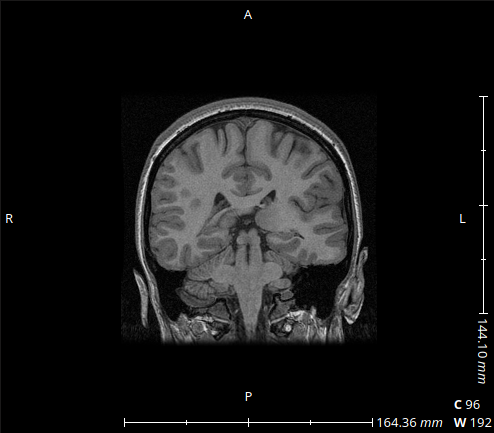
\includegraphics[width=\textwidth]{img/imageorientationindicator-002.png}
        \centering
        \label{fig:imageorientationindicator1}
    \end{figure}
    
    Każda z sześciu możliwych liter oznacza kierunek oraz zwrot w jakim jest ułożony pacjent:
    \begin{itemize}
        \item \quotett{R} - right - część prawa pacjenta
        \item \quotett{L} - left - część 
        \item \quotett{A} - anterior - przód pacjenta
        \item \quotett{P} - posterior - tył pacjenta
        \item \quotett{F} - feet - część dolna
        \item \quotett{H} - head - część górna
    \end{itemize}

    Pary poszczególnych liter tworzą osie:
    \begin{itemize}
        \item \quotett{x} - oś przechodząca od prawej do lewej strony pacjenta, \quotett{L} oznacza zwrot zgodny z osią, a \quotett{R} oznacza zwrot przeciwny, wizualizacja na rysunku \ref{fig:imageorientationindicator2}

        \begin{figure}[h]
            \caption{Wizualizacja osi \quotett{x} pacjenta}
            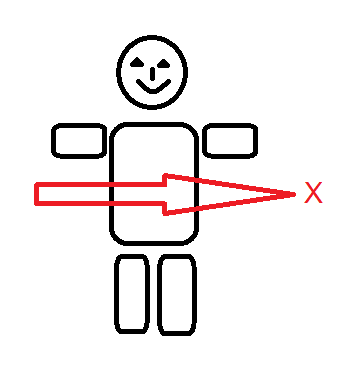
\includegraphics[]{img/imageorientationindicator-101.png}
            \centering
            \label{fig:imageorientationindicator2}
        \end{figure}

        \item \quotett{y} - oś przechodząca od przodu do tył pacjenta, \quotett{P} oznacza zwrot zgodny z osią, a \quotett{A} oznacza zwrot przeciwny, wizualizacja na rysunku \ref{fig:imageorientationindicator3}

        \begin{figure}[h]
            \caption{Wizualizacja osi \quotett{y} pacjenta}
            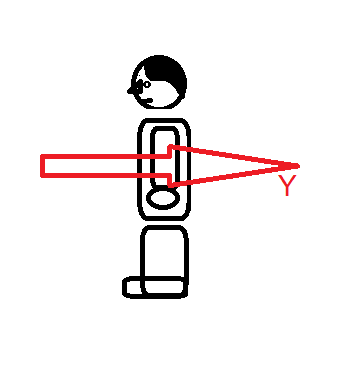
\includegraphics[]{img/imageorientationindicator-102.png}
            \centering
            \label{fig:imageorientationindicator3}
        \end{figure}

        \item \quotett{z} -  - oś przechodząca od dołu do góry pacjenta, \quotett{H} oznacza zwrot zgodny z osią, a \quotett{F} oznacza zwrot przeciwny, wizualizacja na rysunku \ref{fig:imageorientationindicator4}

        \begin{figure}[h]
            \caption{Wizualizacja osi \quotett{z} pacjenta}
            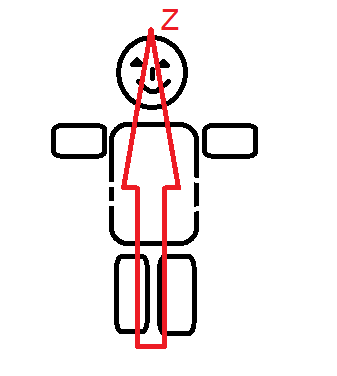
\includegraphics[]{img/imageorientationindicator-103.png}
            \centering
            \label{fig:imageorientationindicator4}
        \end{figure}

    \end{itemize}

    Informacje o orientacji oraz pozycji względem pacjenta znajdują się w odpowiednio w tagach \dicomtag{ImageOrientation}{0020}{0037} i \dicomtag{ImagePosition}{0020}{0032}.
    Wartość \dicomtag{ImageOrientation}{0020}{0037} składa się z sześciu liczb, opowiednio oznaczanych dalej X\textsubscript{x}, X\textsubscript{y}, X\textsubscript{z}, Y\textsubscript{x}, Y\textsubscript{y}, Y\textsubscript{z}.

    Standard DICOM definiuje, że te dane mają być z interpretowane w następujący sposób:    
    \[
        \begin{bmatrix}
            P_x \\ P_y \\ P_z \\ 1
        \end{bmatrix}
        =
        \begin{bmatrix}
            X_x\Delta_i & Y_x\Delta_j & 0 & S_x \\
            X_y\Delta_i & Y_y\Delta_j & 0 & S_y \\
            X_z\Delta_i & Y_z\Delta_j & 0 & S_z \\
            0 & 0 & 0 & 1
        \end{bmatrix}
        \begin{bmatrix}
            i \\ j \\ 0 \\ 1
        \end{bmatrix}
        =
        M
        \begin{bmatrix}
            i \\ j \\ 0 \\ 1
        \end{bmatrix}
    \]
    gdzie:
    \begin{conditions}
    P_{xyz} & The coordinates of the voxel (i,j) in the frame's image plane in units of mm.\\
    S_{xyz} & The three values of Image Position (Patient) (0020,0032). It is the location in mm from the origin of the RCS.\\
    X_{xyz} & The values from the row (X) direction cosine of Image Orientation (Patient) (0020,0037).\\
    Y_{xyz} & The values from the column (Y) direction cosine of Image Orientation (Patient) (0020,0037).\\
    i & Column index to the image plane. The first column is index zero.\\
    \Delta_i & Column pixel resolution of Pixel Spacing (0028,0030) in units of mm.\\
    j & Row index to the image plane. The first row index is zero.\\    
    \Delta_j & Row pixel resolution of Pixel Spacing (0028,0030) in units of mm.
    \end{conditions}

    Brak tłumaczenia jest celowy, aby uniknąć nie porozumień.

    Wyjaśnienia:
    \begin{itemize}
        \item $P_{xyz}$ oznacza punkt pozycji pacjenta wyrażony w milimetrach
        \item $S_{xyz}$ oznacza punkt pozycji pacjenta wyrażony w milimetrach w stosunku do urządzenia wykonującego pomiar, dane brane z \dicomtag{ImagePosition}{0020}{0032}
        \item $X_{xyz}$ oznacza trzy pierwsze wartości z \dicomtag{ImageOrientation}{0020}{0037}
        \item $Y_{xyz}$ oznacza trzy ostatnie wartości z \dicomtag{ImageOrientation}{0020}{0037}
        \item $i$ i $j$ oznaczają współrzędne na obrazu
        \item $\Delta_i$ i $\Delta_j$ oznaczają rzeczywistą wielkość piksela obrazu wyrażoną w mm, w algorytmie wyznaczania strony pacjenta ta wartość, może wynosić 1, ponieważ odpowiada za skale
    \end{itemize}

    Praktycznie rzecz biorąc, pierwsza macierz to wektor reprezentujący pozycje pacjenta.
    Druga jest to transformata.
    Trzecia to pozycja na obrazie.
    
    Interesuje nas wyznaczenie pozycji sześciu (punktów) na płaszczyźnie obrazu, o następujących współrzędnych, dalej używanych pod nazwą $PatientPosition$:
    \begin{itemize}
        \item \quotett{R} - $[-1, 0, 0, 1]$
        \item \quotett{L} - $[+1, 0, 0, 1]$
        \item \quotett{A} - $[0, -1, 0, 1]$
        \item \quotett{P} - $[0, +1, 0, 1]$
        \item \quotett{F} - $[0, 0, -1, 1]$
        \item \quotett{H} - $[0, 0, +1, 1]$
    \end{itemize}

    UWAGA: Wszystkie obliczenia odbywają się w współrzędnych jednorodnych.

    Wykonuje takie przekształcenie:
    \[PatientPosition = imgMatrix * ScenePosition\]
	\[imgMatrix^{-1} * PatientPosition = imgMatrix^{-1} * imgMatrix * ScenePosition\]
	\[imgMatrix^{-1} * PatientPosition = ScenePosition\]
    \[ScenePosition = imgMatrix^{-1} * PatientPosition\]
    gdzie:
    \begin{conditions}
        imgMatrix & macierz przekształcenia obrazu, o której będzie dalej\\
        ScenePosition & pozycja na obrazie, która naz interesuje \\
        PatientPosition & któryś z punktów względem pacjenta.
    \end{conditions}

    Wygląd macierzy $imgMatrix$:
    \[
        \begin{bmatrix}
            X_x & Y_x & 0 & 0 \\
            X_y & Y_y & 0 & 0 \\
            X_z & Y_z & 0 & 0\\
            0 & 0 & 0 & 1
        \end{bmatrix}
    \]
    Powyższa macierz różni się od macierzy definiowanej w standardzie.
    Po pierwsze PikselSpacing został pominięty, a konkretniej nadałem mu wartość 1.
    Po drugie pozycja z \dicomtag{ImagePosition}{0020}{0032} została zrównana do punktu zerowego, dzięki temu, wynik też będzie względem punktu zero.
    Wyznaczenie macierzy $imgMatrix$ jest jednorazowe.

    Po wyznaczeniu sześciu punktów $ScenePosition$, po jednej dla każdego punktu względem pacjenta są zapisywane. $ScenePosition$ odpowiada pozycji punktów na obrazie w pozycji startowej.

    Na scenie, której jest wyświetlany obraz, użytkownik, może obracać obraz do woli, według własnego uznania.
    Te przekształcenia, są realizowane za pomocą macierzy rotacji, dalej znana jako $rotateTransform$.
    Macierz $rotateTransform$ jest przesyłana do naszego obiektu \sokarclass{ImageOrientationIndicator} za każdym razem kiedy zostanie zmieniona.

    Ostateczne wyznaczenie pozycji punktów pacjent na obrazie odbywa sie przez przemnożenie lewostronne $rotateTransform$ i $ScenePosition$.
    \[rotateTransform * ScenePosition\]
    Wyznaczane jest w ten sposób pozycja sześciu punktów pacjenta na płaszczyźnie sceny wyświetlanej.
    Następnie określane jest na, której z ośmiu części płaszczyzny jest umieszczony dany punkt, podział płaszczyzny jest widoczny na rysunku \ref{fig:imageorientationindicator5}.
    Tej płaszczyźnie nadawany jest tytuł w postaci litery, która oznacza punkt pacjenta.
    Jeżeli punkt znajduje się w centrum, na przecięciu osi, to oznacza, że punkt znajduje się za lub przed ekranem, więc jest pomijany.
    Następnie do czterech pól wyświetlających zostają wstawione następujące teksty:
    \begin{itemize}
        \item lewe pole: tytuł części 7, tytuł części 0 i tytuł części 1
        \item górne pole: tytuł części 1, tytuł części 2 i tytuł części 3
        \item prawe pole: tytuł części 3, tytuł części 4 i tytuł części 5
        \item dolne pole: tytuł części 7, tytuł części 6 i tytuł części 5
    \end{itemize}

    Przykład:\\
    Punkt \quotett{H}, czyli punkt reprezentujący kierunek głowy, został przypisany do części 1 i odpowiednio \quotett{L} do części 7, \quotett{R} do części 3 i \quotett{F} do części 5.
    Punkty \quotett{A} i \quotett{P} zostały pominięte ponieważ znalazły się na środku.
    Do lewego pola wstawiany jest tekst \quotett{HL}, do górnego \quotett{HR}, do prawego \quotett{RF} i do dolnego \quotett{LF}.

    \begin{figure}[h]
        \caption{Podział płaszczyzny sceny. Wyróżniono osiem części.}
        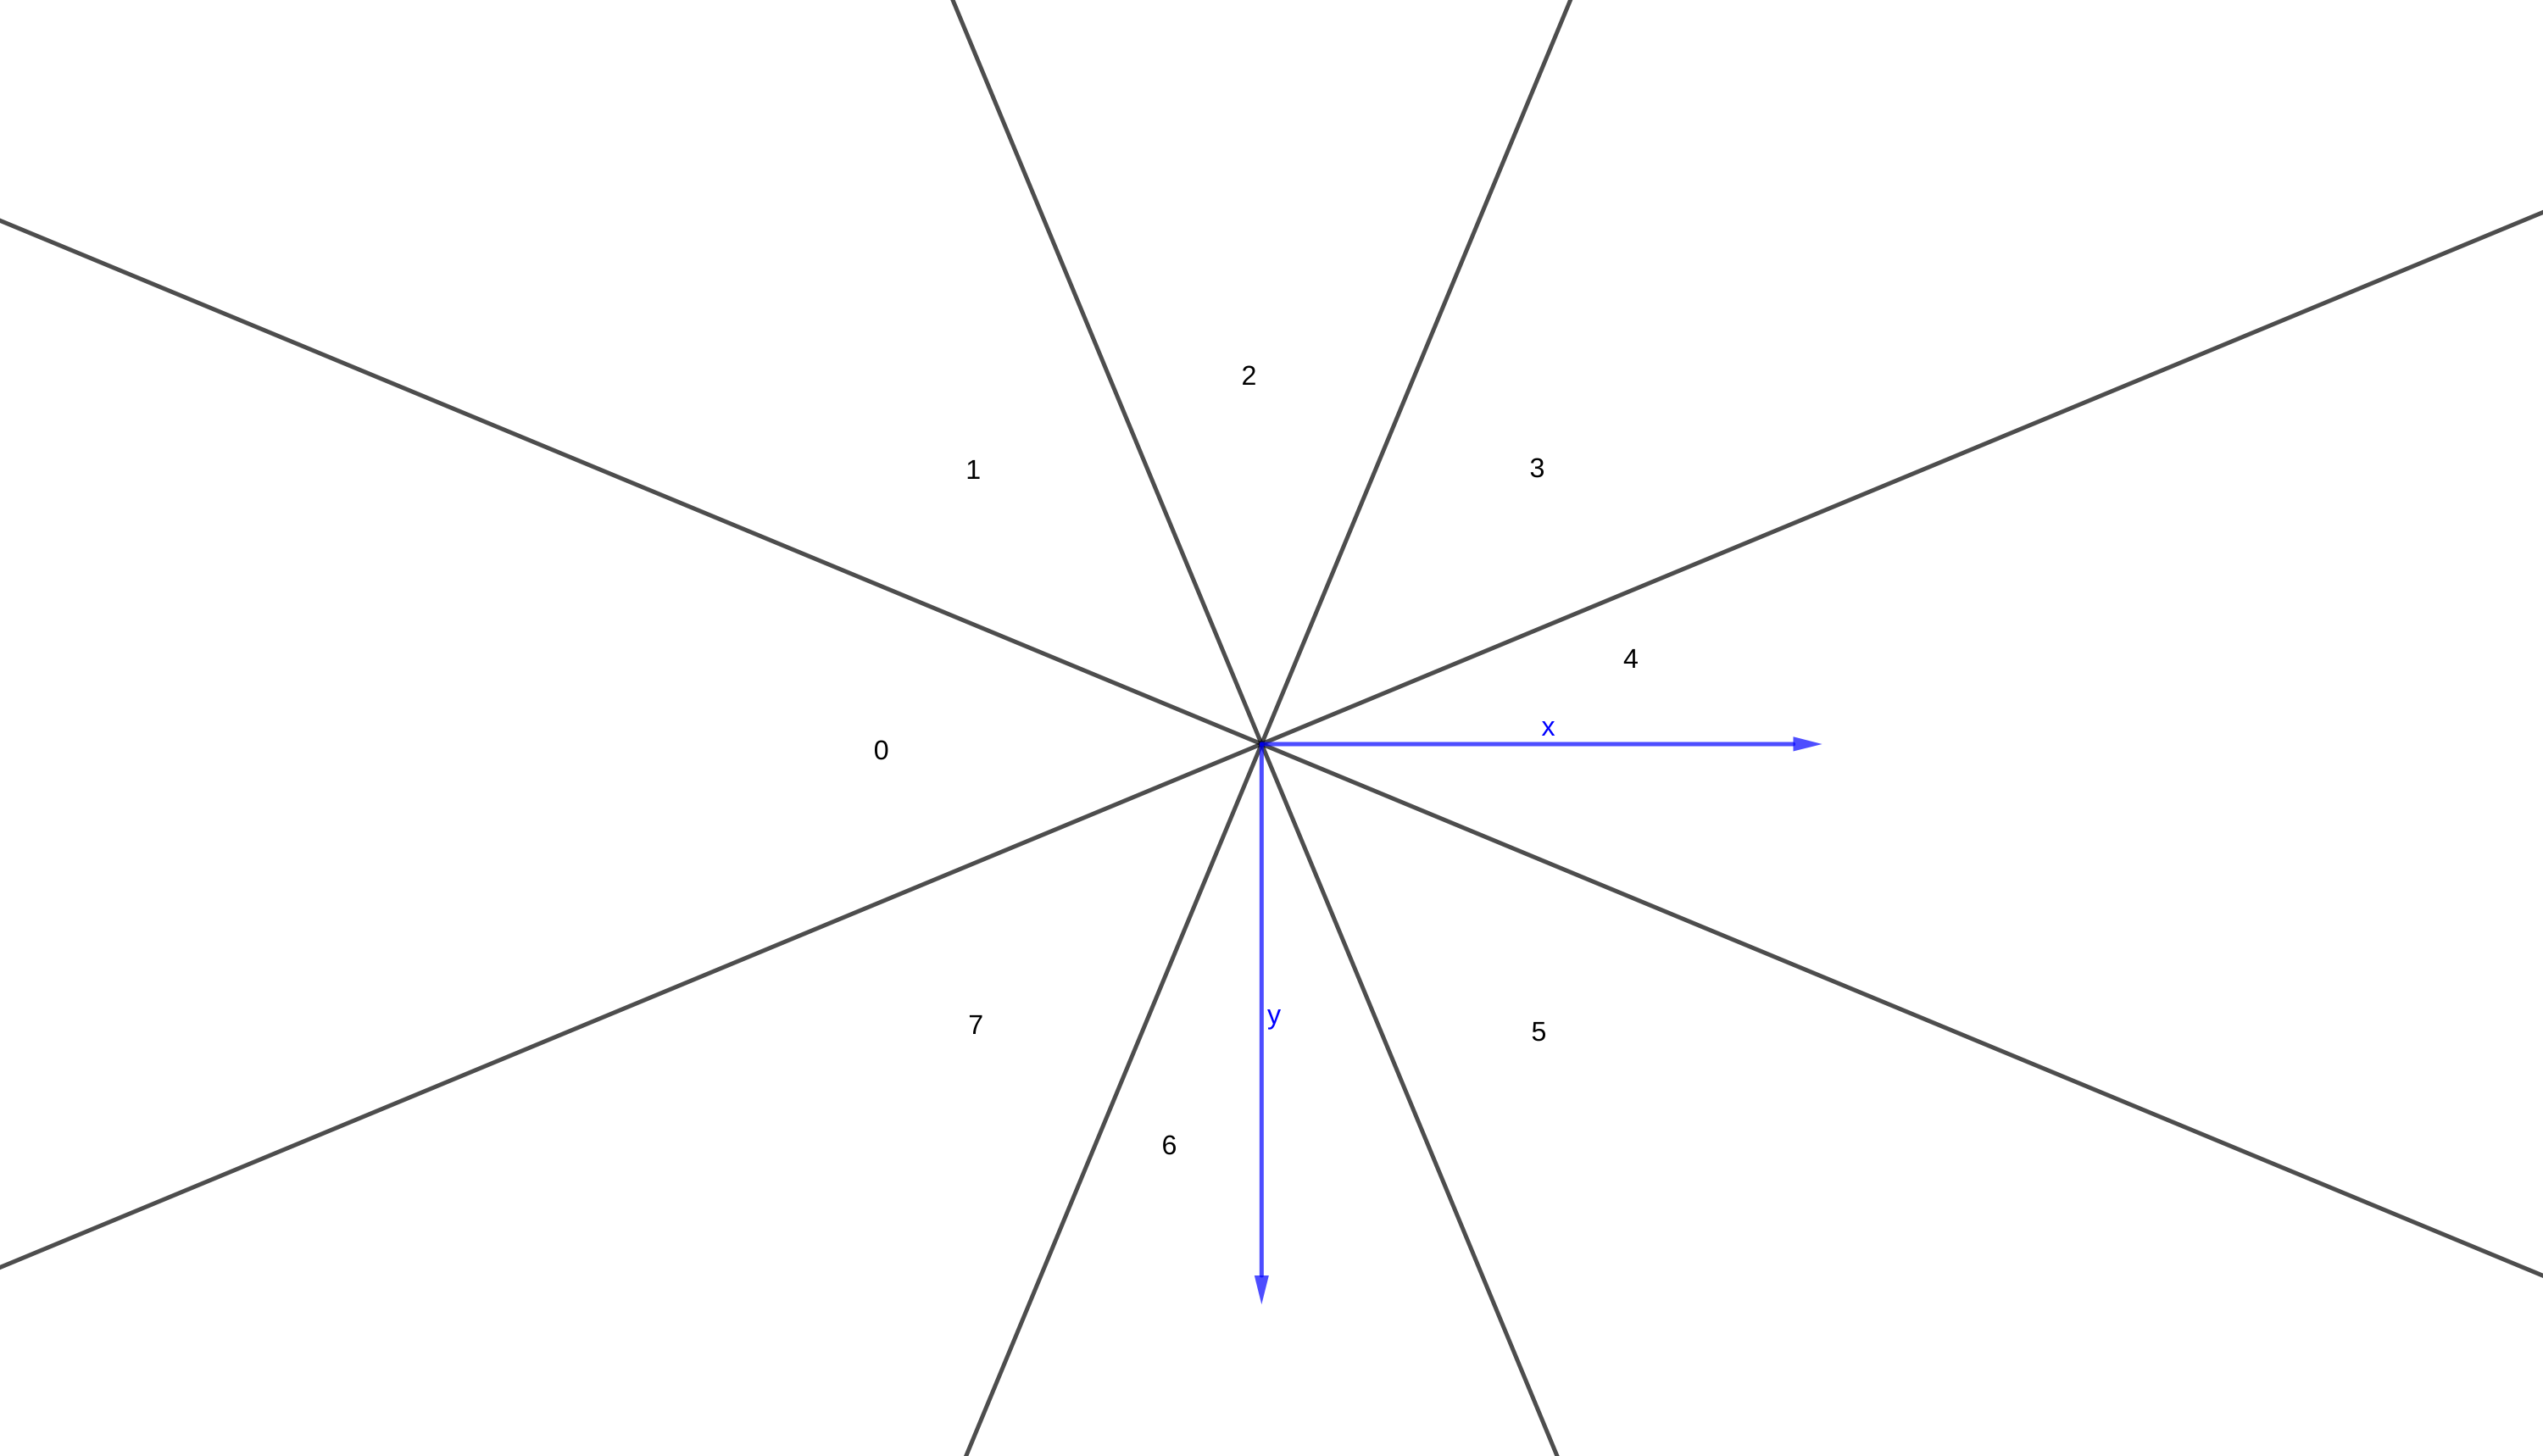
\includegraphics[width=\textwidth]{img/imageorientationindicator-300.png}
        \centering
        \label{fig:imageorientationindicator5}
    \end{figure}

    \item \sokarclass{PixelSpacingIndicator}
    
    Obiekt wyświetlający miarkę z podziałką informującą jakich rozmiarów jest obiekt na obrazie w rzeczywistości, pojawia się na dole i po prawie stronie sceny, gdy tag \dicomtag{PixelSpacing}{0028}{0030} jest obecny.
    Wygląd podziałki można zaobserwować na rysunku \ref{fig:imageorientationindicator1}.

    Podziałka dostosowuje swoją wielkość do obecnej sceny, jak i do innych elementów na scenie.
    Wartości wyświetlane biorą pod uwagę transformatę skali i rotacji obrazu.

    \item \sokarclass{ModalityIndicator}
    
    Obiekt wyświetla informacje o akwizycji obrazu.
    Dane różnią się w zależności od modalności obrazu.
    Domyślnie zawierają następujące linie:
    \begin{itemize}
        \item bla bla bla
        \item bla bla bla
        \item bla bla bla
        \item bla bla bla
    \end{itemize}

    W przypadku następujących modalności zawierają również następujące informacje:
    \begin{itemize}
        \item bla bla bla
        \item bla bla bla
        \item bla bla bla
        \item bla bla bla
    \end{itemize}
\end{itemize}


\subsection{Generowanie obrazów z danych}

Klasa \sokarclass{DicomScene} jest klasą abstrakcyjną i nie generuje obrazu, pozostawia do klasą dziedziczących po niej.

\paragraph{Cykl generowania obrazu}

Klasa \sokarclass{DicomScene} dostarcza następujące obiekty do generowania obrazu:
\begin{itemize}
    \item \cppcode{QMutex processing} mutex do zablokowania podczas generowania obrazu, aby parametry obrazu nie mogły być zmienianie podczas jego generowania.
    
    \item \cppcode{uint imgDimX} szerokość obrazu w pikselach.
    
    \item \cppcode{uint imgDimY} wysokość obrazu w pikselach.
    
    \item \cppcode{std::vector<Pixel> targetBuffer} wektor docelowego obrazu RGB o długości $imgDimX*imgDimY$.
    
    \cppcode{Pixel} to struktura reprezentujące piksel, wyglądające następująco:
    
    \cppcode{struct Pixel \{ quint8 red = 0, green = 0, blue = 0; \};}

    \item \cppcode{std::vector<char> originBuffer} wektor danych wypełniona danymi z jednej ramki o długośći iloczynu $imgDimX*imgDimY$ i ilości bajtów jednego piksela obrazu.

    \item \cppcode{QImage qImage} obiekt obrazu.
    
    \qtclass{QImage} można zrobić z istniejącego bufora, w tym przypadku jest to \cppcode{targetBuffer}.
    Format obrazu to \qtclass{QImage::Format\_RGB888}, czyli trzy bajty, każdy na jeden kanał.

    \item \cppcode{QPixmap pixmap} obiekt obrazu do wyświetlania.
    
    Obiektów klasy \qtclass{QImage} nie da się wyświetlić, nie jest on przystosowany do wyświetlania.
    Natomiast klasa \qtclass{QPixmap} to reprezentacja obrazu dostosowana do wyświetlania ekranie, która może być używana jako urządzenie do malowania w bibliotece Qt.

    \item \cppcode{QPixmap iconPixmap} obiekt obrazu ikonu, docelowo powinien mieć 128 pikseli na 128 pikseli.
    
    \item \cppcode{QGraphicsPixmapItem *pixmapItem} wskaźnik do obiektu na scenie, który wyświetla \cppcode{pixmap}.
    
\end{itemize}

Generowanie obrazu jest robione przez funkcje \sokarclass{DicomScene::generatePixmap()}.
Po wywołaniu funkcji obiekt \cppcode{pixmap} powinien zawierać obraz wygenerowany z obecnymi parametrami.
Funkcja zwraca również \cppcode{bool}, który informuje nas czy \cppcode{pixmap} rzeczywiście został zmieniony.

Całe odświeżanie obrazu jest implementowane w funkcji \sokarclass{DicomScene::reloadPixmap()}.
Funkcja wywołuje \sokarclass{DicomScene::generatePixmap()} i odświeża \cppcode{pixmapItem} kiedy zajdzie taka potrzeba

Generowanie poszczególnych typów obrazów jest wyjaśnione poniżej.

\subsubsection{Monochorme}
\input{implementation/pixmap-monochrome.tex}

\subsubsection{RGB}
\input{implementation/pixmap-rgb.tex}

\subsubsection{YBR}
\input{implementation/pixmap-ybr.tex}


\section{DicomView}

Każda zakładka z obrazem lub obrazami jest implementowana przez klasę \sokarclass{DicomView}.

Interfejs graficzny \sokarclass{DicomView} posiada następujące elementy:
\begin{itemize}
    \item pasek narzędzi znajdujący się na górze - implementowany za pomocą klasy \sokarclass{DicomToolBar}
    \item miejsce na scene z obrazem DICOM na środku - implementowany za pomocą klasy \sokarclass{DicomGraphics}
    \item suwak filmu w dolnej części - implementowany za pomocą klasy \sokarclass{MovieBar}
    \item podgląd miniaturek obrazów w prawej części - implementowany za pomocą klasy \sokarclass{FrameChooser}
\end{itemize}

Dodatkowo posiada obiekt \sokarclass{DicomSceneSet}, który jest zbiorem obrazów opisany w sekcji \ref{sec:scene-sets}.
\sokarclass{DicomView} łączy zdarzenia wysyłane przez wszystkie obiekty.

Poniżej jest opisane zachowanie tych elementów:

\subsection{Elementy interfejsu graficznego}

\subsubsection{\sokarclass{DicomToolBar}}

Jest to pasek narzędzi znajdujący się na górze \sokarclass{DicomView}.
Posiada on zespół ikonek z rozwijalnymi menu kontekstowymi.
Kliknięcie odpowiedniej ikony spowoduje wysłanie sygnału do obecnie wyświetlanej sceny.

Są dwa sygnału Qt wysyłane przez klase:
\begin{itemize}
    \item \cppcode{void stateToggleSignal(State state);}

    Sygnał ten oznacza zmianę stanu interfejsu

    \item \cppcode{void actionTriggerSignal(Action action, bool state = false);}
\end{itemize}


Ikony na pasku:
\begin{itemize}
    \item Okienkowanie
    \item Przesuwanie
    \item Skalowanie
    \item Rotacja
    \item Indicators
    \item Tagi - czerwona ikonka dwóch metek

    Kliknięcie 
\end{itemize}

\subsubsection{\sokarclass{DicomGraphics}}
\subsubsection{\sokarclass{MovieBar}}
\subsubsection{\sokarclass{FrameChooser}}

\subsection{Zależności pomiędzy elementami graficznymi}

\section{Tryb filmu - MovieMode}
\label{sec:scene-sets}

Przeglądarka obsługuje możliwość wyświetlenia sekwencji obrazu i stworzenia czegoś na kształt filmu.

Na początku należy ustalić z czego ten film chcemy.

\paragraph{Tworzenie zestawu obrazów}


\subparagraph{Tworzenie zestawu obrazów z jednego pliku}



\subparagraph{Tworzenie zestawu obrazów z wielu plików}

Zawsze kiedy otwieramy pliki, tworzona jest wektor tych plików, gdy otwieramy jeden plik jest to wektor z jednym elementem.
Po wczytaniu plików, funkcja \sokarclass{DicomFileSet::create()} dzieli wektor na 

Istnieje możliwość 


\end{document}
